    \section{Présentation du sujet}


\begin{frame}
\frametitle{Présentation du sujet}
\begin{itemize}
    \itemsep2em
    \item Boulangerie
    \item Portée globale
    \item Réseau fermé
    \item Gestion de commerce
\end{itemize}
\end{frame}



    \section{Analyse}


\subsection{Stocks}
\begin{frame}
\frametitle{Stocks}
\begin{itemize}
    \itemsep2em
    \item Matières premières liées aux produits
    \item Produits éphémères
    \item Matières premières en flux tendu % Péremption non prise en compte
\end{itemize}
\end{frame}

\subsection{Commerce}
\begin{frame}
\frametitle{Commerce}
\begin{itemize}
    \itemsep2em
    \item Ventes immédiates en magasin
    \item Commandes différées
\end{itemize}
\end{frame}

\subsection{Intervenants}
\begin{frame}
\frametitle{Intervenants}
\begin{itemize}
    \itemsep2em
    \item Clients optionnellement enregistrés
    \item Fournisseurs enregistrés
\end{itemize}
\end{frame}


    \section{Cahier des charges}

\subsection{Stocks}
\begin{frame}
\frametitle{Stocks}
\begin{itemize}
    \itemsep2em
    \item Matière premières
    \item Produits
\end{itemize}
\end{frame}

\subsection{Commerce}  % Partie Anthony
\begin{frame}
\frametitle{Commerce}
\begin{itemize}
    \itemsep2em
    \item Ventes
    \item Commandes
\end{itemize}
\end{frame}

\subsection{Intervenants}
\begin{frame}
\frametitle{Intervenants}
\begin{itemize}
    \itemsep2em
    \item Fournisseurs
    \item Clients
\end{itemize}
\end{frame}


    \section{Réalisation}


\subsection{Tableau de bord}
\begin{frame}
\frametitle{Tableau de bord}
\begin{figure}[h!]
    \centerline{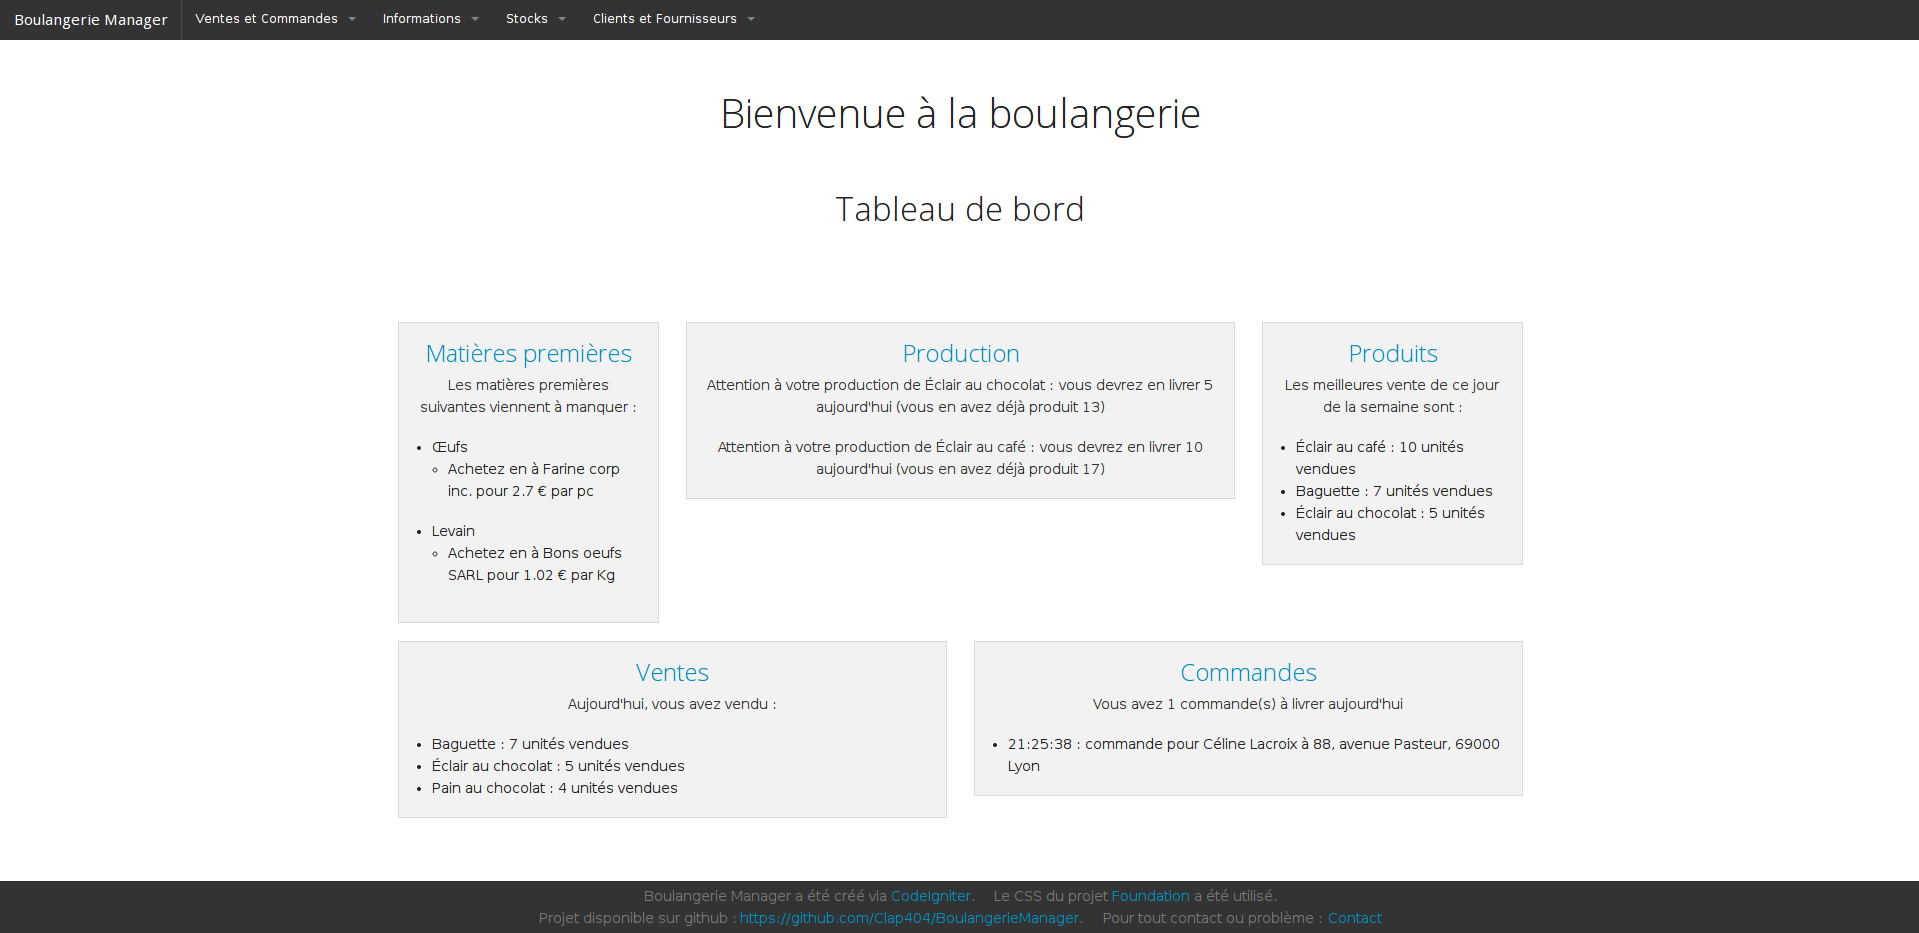
\includegraphics[width=1\textwidth]{images/tableau_de_bord.png}}
    \caption{Tableau de bord}
\end{figure}
\end{frame}

\subsection{Statistiques}
\begin{frame}
\frametitle{Statistiques}
\begin{figure}[h!]
    \centerline{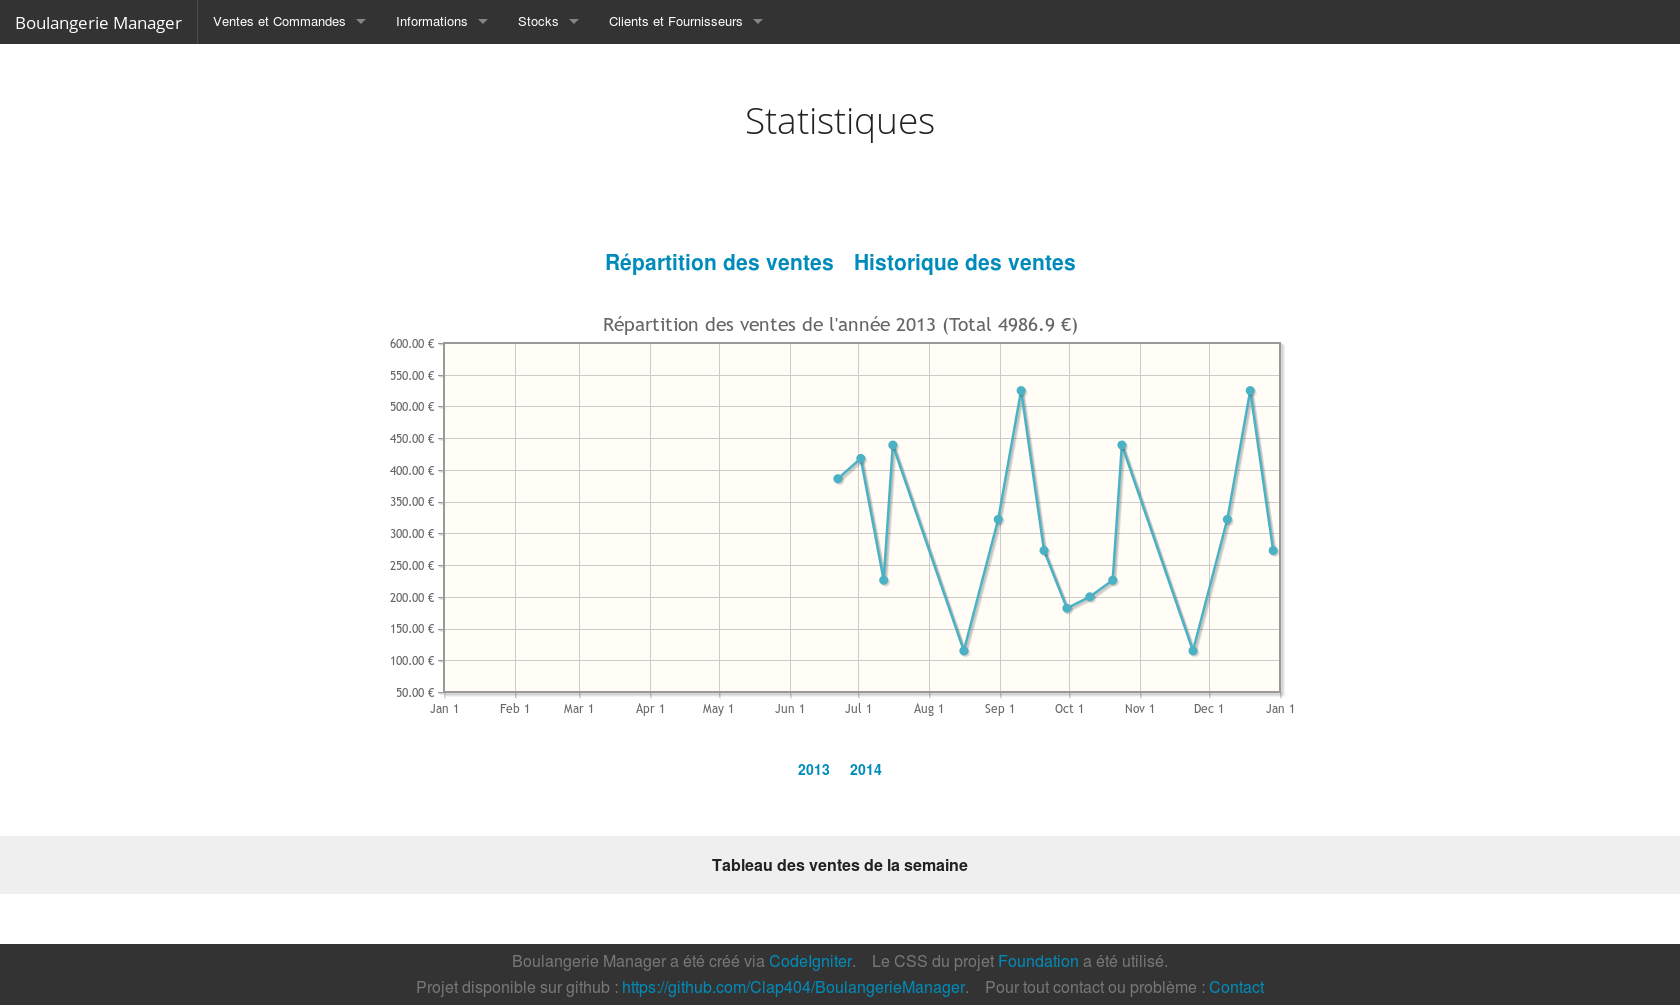
\includegraphics[width=0.85\textwidth]{images/stats.png}}
    \caption{Statistiques}
\end{figure}
\end{frame}

\subsection{Ventes}
\begin{frame}
\frametitle{Ventes}
\begin{figure}[h!]
    \centerline{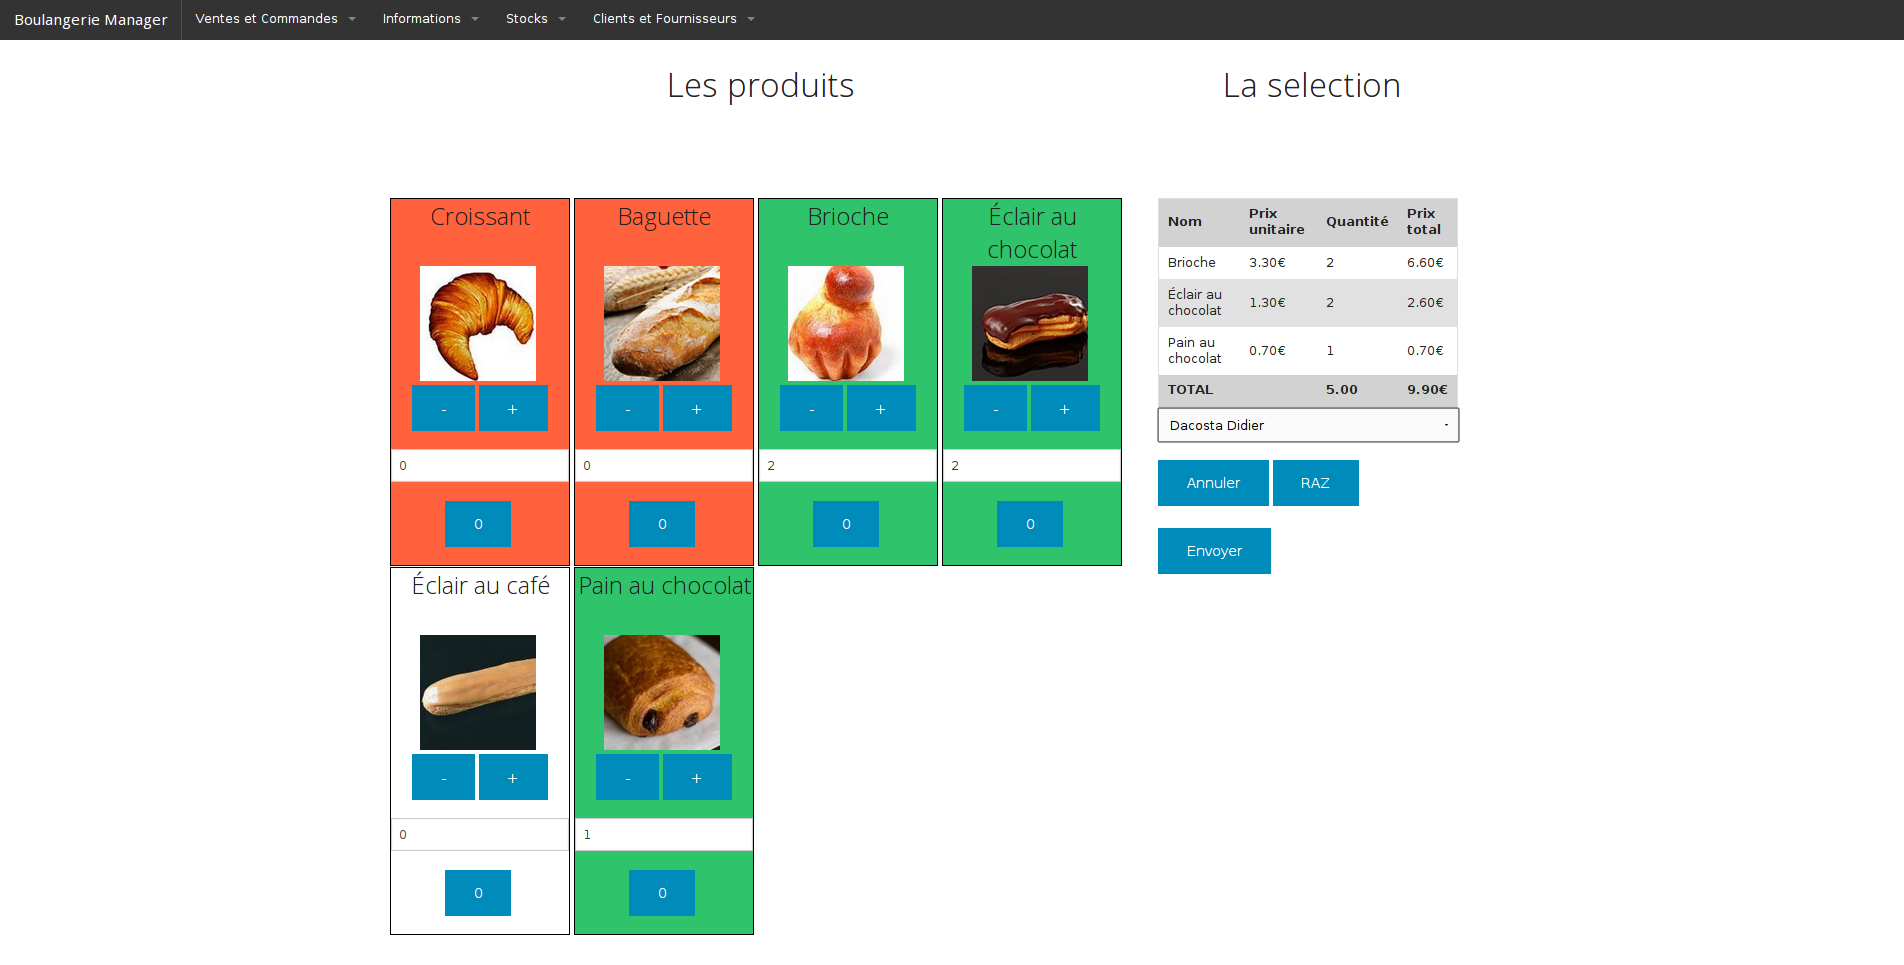
\includegraphics[width=1\textwidth]{images/ventes.png}}
    \caption{Ventes}
\end{figure}
\end{frame}

\subsection{Clients}
\begin{frame}
\frametitle{Clients}
\begin{figure}[h!]
    \centerline{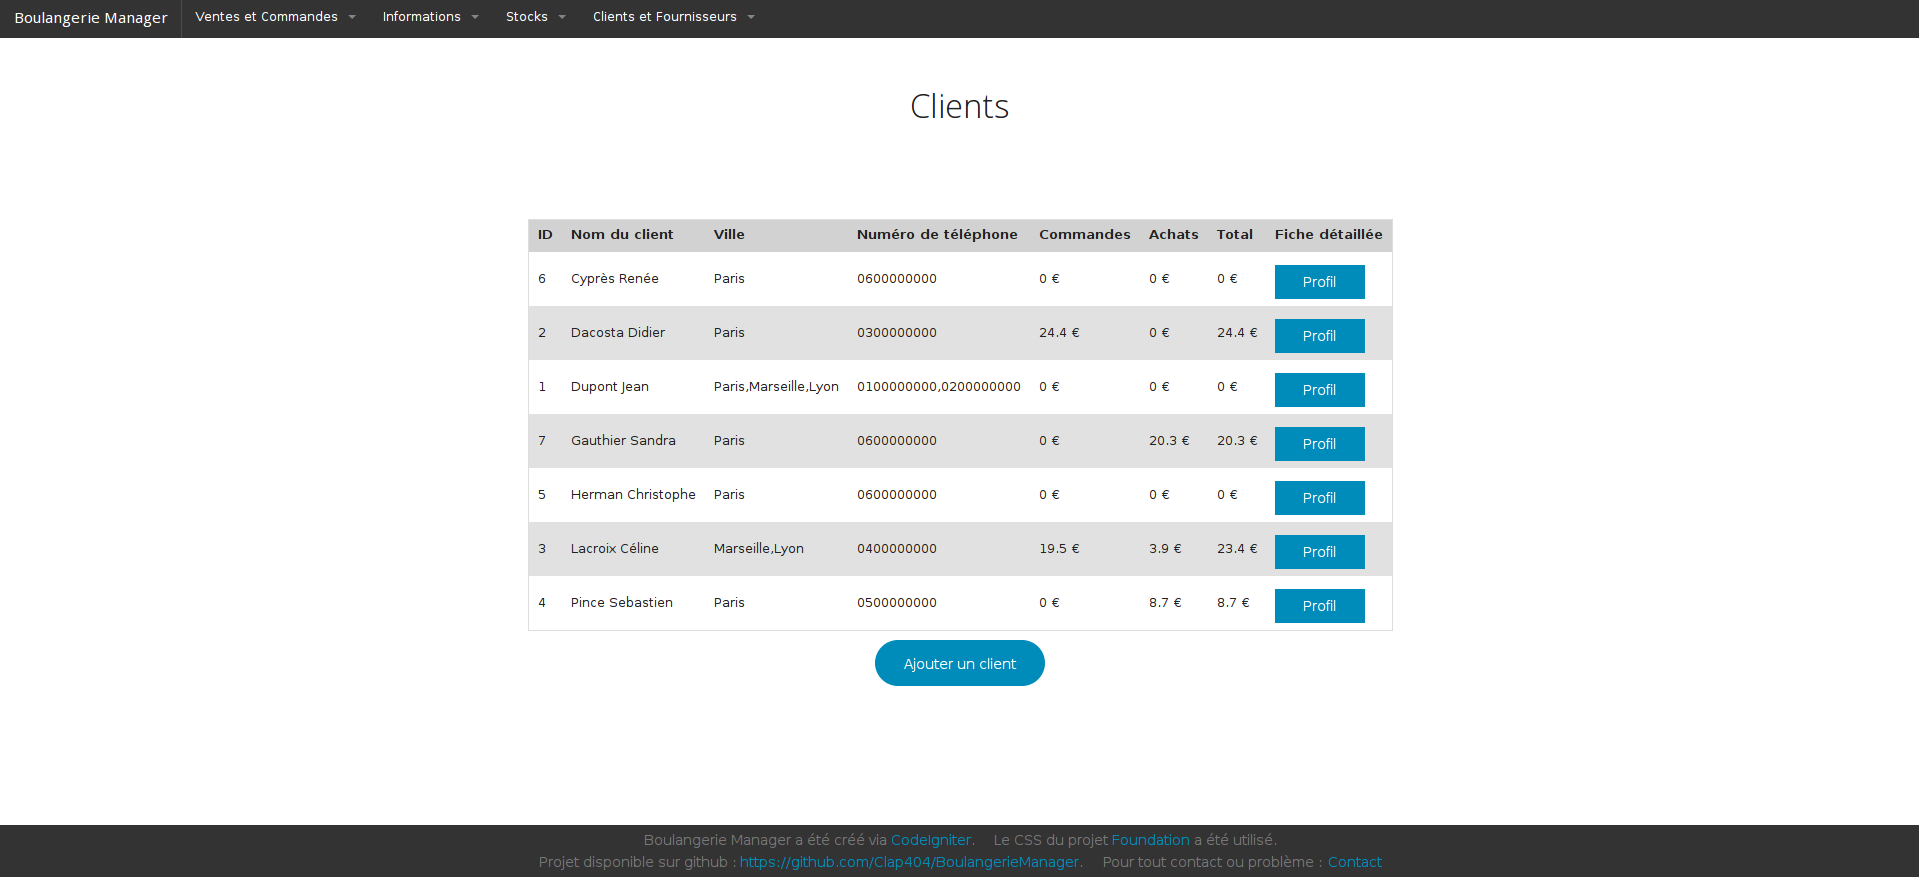
\includegraphics[width=1\textwidth]{images/clients.png}}
    \caption{Clients}
\end{figure}
\end{frame}


    \section{Planning et répartition des tâches}


\subsection{Planning}
\begin{frame}
\frametitle{Planning}
\begin{center}
\begin{figure}[h!]
    \centering
    \begin{tabular}{|l|l|}
        \hline
        18/10/2013 & MCD terminé. \\
        \hline
        28/10/2013 & Début du développement. \\
        \hline
        Novembre 2013 & Interface réalisée, base de donnée créée. \\
        \hline
        \multirow{2}{*}{Décembre 2013}
            & Site fonctionnel, design proche du rendu final. \\
            & Début de la phase de corrections de bugs. \\
        \hline
        07/01/2014 & Finalisation du développement. \\
        \hline
    \end{tabular}
    \caption{Planning du projet}
\end{figure}
\end{center}
\end{frame}

\subsection{Répartition des tâches}
{
\logo{}
\begin{frame}
\frametitle{Répartition des tâches}
\begin{center}
\begin{figure}[h!]
    \centering
    \begin{tabular}{|l|l|}
        \hline
            Jérémy Autran & Parties ventes et commandes. Page d'accueil.\\
        \hline
            Florian Barrois & Parties statistiques. \\
        \hline
            François-Xavier Béligat & Partie produits. \\
        \hline
            Maxime Chenot & Organisation graphique et design. \\
        \hline
            Arnaud Colin & Parties statistiques. \\
        \hline
            Benoît Houdayer & Parties fournisseurs et clients. \\
        \hline
            \multirow{2}{*}{Anthony Ruhier} & Partie matières premières. Partie
            invendus.\\
            & Partie statistiques.\\
        \hline
    \end{tabular}
    \caption{Répartition des tâches}
\end{figure}
\end{center}
\end{frame}
}


    \section{Conclusion}


\begin{frame}
\frametitle{Conclusion}
\centering \Large{Des questions ?\\[2em]}

\small{Projet disponible sur Github :}
{\color{blue}\url{github.com/Clap404/BoulangerieManager/}}
\end{frame}
